\documentclass[border=1pt]{standalone}
\usepackage[T1]{fontenc}
\usepackage{txfonts}
\usepackage{xcolor}
\usepackage{tikz}
\usetikzlibrary{arrows.meta,positioning,calc,fit,backgrounds,patterns,decorations.pathreplacing}
\usepackage{pgfplots}
\pgfplotsset{compat=1.17, scaled ticks=false}
\usepgfplotslibrary{fillbetween}
\newcommand{\us}{u_{\mathrm{s}}}
\newcommand{\ue}{u_{\mathrm{e}}}
\newcommand{\tc}{\tau_c}
\newcommand{\tstar}{\tau^{*}}
\newcommand{\expl}{$^{\dagger}$}
% text and lines
\definecolor{ink}{HTML}{1F2937}
\definecolor{boxfill}{HTML}{F3F4F6}
% detections (Okabe-Ito): correct blue, wrong vermilion
\definecolor{corr}{HTML}{0072B2}
\definecolor{wrng}{HTML}{D55E00}
% outcomes (colour-blind and greyscale safe)
\definecolor{appc}{HTML}{009E73}  % applicable
\definecolor{ndc}{HTML}{F0E442}   % not determined
\definecolor{nac}{HTML}{882255}   % not applicable
\definecolor{ntc}{HTML}{FFFFFF}   % no threshold selected
\definecolor{edge}{HTML}{7F7F7F}
\definecolor{expfill}{HTML}{EFEFEF}

\begin{document}
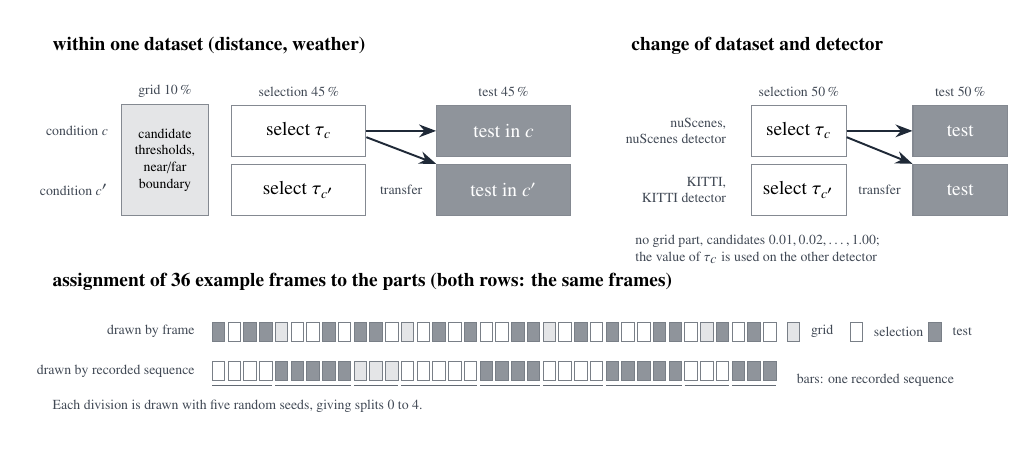
\begin{tikzpicture}[font=\scriptsize, >=Stealth,
  cell/.style={draw=ink!55, line width=0.4pt, minimum height=6.5mm, inner sep=1pt, align=center},
  head/.style={font=\scriptsize\bfseries, anchor=south west},
  lab/.style={font=\tiny, text=ink!85}]
% ================= left block: within one dataset
\node[head] at (0,1.30) {within one dataset (distance, weather)};
% column heads
\node[lab] at (1.55,0.95) {grid 10\,\%};
\node[lab] at (3.25,0.95) {selection 45\,\%};
\node[lab] at (5.85,0.95) {test 45\,\%};
% rows
\node[lab, anchor=east] at (0.95,0.45) {condition $c$};
\node[lab, anchor=east] at (0.95,-0.30) {condition $c'$};
\node[cell, fill=ink!12, minimum width=11mm, minimum height=14mm, text width=10mm, font=\tiny] at (1.55,0.08) {candidate thresholds, near/far boundary};
\node[cell, fill=white, minimum width=17mm] (sc) at (3.25,0.45) {select $\tc$};
\node[cell, fill=white, minimum width=17mm] (sc2) at (3.25,-0.30) {select $\tau_{c'}$};
\node[cell, fill=ink!50, text=white, minimum width=17mm] (ec) at (5.85,0.45) {test in $c$};
\node[cell, fill=ink!50, text=white, minimum width=17mm] (ec2) at (5.85,-0.30) {test in $c'$};
\draw[->, ink, line width=0.7pt] (sc.east) -- (ec.west);
\draw[->, ink, line width=0.7pt] ($(sc.east)+(0,-0.08)$) -- (ec2.north west);
\node[lab] at (4.55,-0.30) {transfer};
% ================= right block: between datasets
\begin{scope}[shift={(7.35,0)}]
\node[head] at (0,1.30) {change of dataset and detector};
\node[lab] at (2.25,0.95) {selection 50\,\%};
\node[lab] at (4.30,0.95) {test 50\,\%};
\node[lab, anchor=east, align=right] at (1.45,0.45) {nuScenes,\\ nuScenes detector};
\node[lab, anchor=east, align=right] at (1.45,-0.30) {KITTI,\\ KITTI detector};
\node[cell, fill=white, minimum width=12mm] (sn) at (2.25,0.45) {select $\tc$};
\node[cell, fill=white, minimum width=12mm] (sk) at (2.25,-0.30) {select $\tau_{c'}$};
\node[cell, fill=ink!50, text=white, minimum width=12mm] (en) at (4.30,0.45) {test};
\node[cell, fill=ink!50, text=white, minimum width=12mm] (ek) at (4.30,-0.30) {test};
\draw[->, ink, line width=0.7pt] (sn.east) -- (en.west);
\draw[->, ink, line width=0.7pt] ($(sn.east)+(0,-0.08)$) -- (ek.north west);
\node[lab] at (3.275,-0.30) {transfer};
\node[lab, align=left, anchor=north west] at (0.05,-0.75) {no grid part, candidates $0.01, 0.02, \dots, 1.00$;\\ the value of $\tc$ is used on the other detector};
\end{scope}
% ================= bottom strip: how frames are drawn
\begin{scope}[shift={(0,-1.75)}]
\node[head] at (0,0.05) {assignment of 36 example frames to the parts (both rows: the same frames)};
\pgfmathsetseed{7}
% drawn by frame: random part per frame
\node[lab, anchor=east] at (2.05,-0.35) {drawn by frame};
\foreach \k/\p in {1/2,2/1,3/2,4/2,5/0,6/1,7/1,8/2,9/1,10/2,11/2,12/1,13/0,14/1,15/2,16/1,17/2,18/1,19/1,20/2,21/2,22/0,23/1,24/2,25/1,26/2,27/1,28/1,29/2,30/2,31/1,32/0,33/2,34/1,35/2,36/1}{
  \ifnum\p=0 \def\ff{ink!12}\fi \ifnum\p=1 \def\ff{white}\fi \ifnum\p=2 \def\ff{ink!50}\fi
  \filldraw[fill=\ff, draw=ink!60, line width=0.3pt] ({2.15+(\k-1)*0.2},-0.47) rectangle ++(0.16,0.24);}
% drawn by recorded scene: runs of frames share a part
\node[lab, anchor=east] at (2.05,-0.85) {drawn by recorded sequence};
\foreach \k/\p in {1/1,2/1,3/1,4/1,5/2,6/2,7/2,8/2,9/2,10/0,11/0,12/0,13/1,14/1,15/1,16/1,17/1,18/2,19/2,20/2,21/2,22/1,23/1,24/1,25/1,26/2,27/2,28/2,29/2,30/2,31/1,32/1,33/1,34/2,35/2,36/2}{
  \ifnum\p=0 \def\ff{ink!12}\fi \ifnum\p=1 \def\ff{white}\fi \ifnum\p=2 \def\ff{ink!50}\fi
  \filldraw[fill=\ff, draw=ink!60, line width=0.3pt] ({2.15+(\k-1)*0.2},-0.97) rectangle ++(0.16,0.24);}
\foreach \a/\b in {1/4,5/9,10/12,13/17,18/21,22/25,26/30,31/33,34/36}{
  \draw[ink!70, line width=0.4pt] ({2.15+(\a-1)*0.2},-1.03) -- ({2.15+(\b-1)*0.2+0.16},-1.03);}
\node[lab, anchor=west] at (9.45,-0.97) {bars: one recorded sequence};
% legend of parts
\filldraw[fill=ink!12, draw=ink!60, line width=0.3pt] (9.45,-0.47) rectangle ++(0.16,0.24); \node[lab, anchor=west] at (9.63,-0.35) {grid};
\filldraw[fill=white, draw=ink!60, line width=0.3pt] (10.25,-0.47) rectangle ++(0.16,0.24); \node[lab, anchor=west] at (10.43,-0.35) {selection};
\filldraw[fill=ink!50, draw=ink!60, line width=0.3pt] (11.25,-0.47) rectangle ++(0.16,0.24); \node[lab, anchor=west] at (11.43,-0.35) {test};
\end{scope}
\node[lab, anchor=west] at (0,-3.05) {Each division is drawn with five random seeds, giving splits 0 to 4.};
\end{tikzpicture}
\end{document}
